%%%%%%%%%%%%%%%%%%%%%%%%%%%%%%%%%%%%%%%%%%%%%%%%%%%%%%%%%%%%%%%%%%%%%%%%%%%
%% This file is part of the book
%%
%% Algorithmic Graph Theory
%% http://code.google.com/p/graph-theory-algorithms-book/
%%
%% Copyright (C) 2009, 2010, 2011 Minh Van Nguyen <nguyenminh2@gmail.com>
%%
%% See the file COPYING for copying conditions.
%%%%%%%%%%%%%%%%%%%%%%%%%%%%%%%%%%%%%%%%%%%%%%%%%%%%%%%%%%%%%%%%%%%%%%%%%%%

\documentclass{article}

\usepackage{subfigure}
\usepackage{tikz}
\usetikzlibrary{external}
\tikzexternalize{mesh-grid-lattice}

\begin{document}

\begin{figure}
%% mesh M(3,4)
\subfigure[$M(3, 4)$]{
\label{fig:introduction:2_mesh_M34}
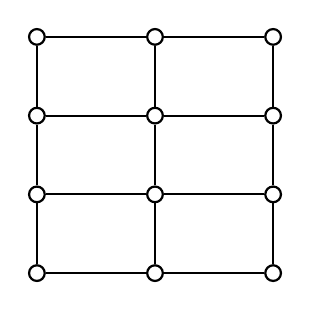
\begin{tikzpicture}
[nodeDecorate/.style={shape=circle,inner sep=2pt,draw,thick},%
  lineDecorate/.style={-,thick}]
%% nodes or vertices
\foreach \nodename/\x/\y in {
  1/0/0,  2/1.5/0,  3/3/0,
  4/0/1,  5/1.5/1,  6/3/1,
  7/0/2,  8/1.5/2,  9/3/2,
  10/0/3, 11/1.5/3, 12/3/3}
{
  \node (\nodename) at (\x,\y) [nodeDecorate] {};
}
%% edges or lines
\path
\foreach \startnode/\endnode in {
  1/4, 4/7, 7/10,
  2/5, 5/8, 8/11,
  3/6, 6/9, 9/12,
  1/2, 2/3, 4/5, 5/6, 7/8, 8/9, 10/11, 11/12}
{
  (\startnode) edge[lineDecorate] node {} (\endnode)
};
\end{tikzpicture}
}
%%
%%
\qquad
%% mesh M(3,2,3)
\subfigure[$M(3, 2, 3)$]{
\label{fig:introduction:3_mesh_M323}
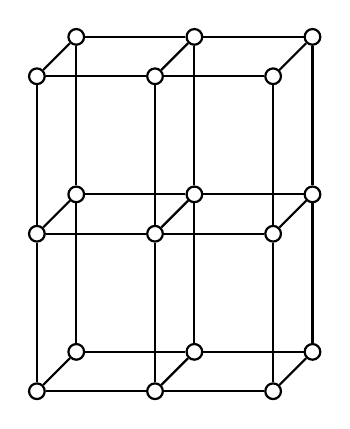
\begin{tikzpicture}
[nodeDecorate/.style={shape=circle,inner sep=2pt,draw,thick},%
  lineDecorate/.style={-,thick}]
%% nodes or vertices
\foreach \nodename/\x/\y in {
  1/0/0,      2/1.5/0,  3/3/0,
  4/0/2,      5/1.5/2,  6/3/2,
  7/0/4,      8/1.5/4,  9/3/4,
  10/0.5/0.5, 11/2/0.5, 12/3.5/0.5,
  13/0.5/2.5, 14/2/2.5, 15/3.5/2.5,
  16/0.5/4.5, 17/2/4.5, 18/3.5/4.5}
{
  \node (\nodename) at (\x,\y) [nodeDecorate] {};
}
%% edges or lines
\path
\foreach \startnode/\endnode in {
  1/2, 2/3, 4/5, 5/6, 7/8, 8/9,
  10/11, 11/12, 13/14, 14/15, 16/17, 17/18,
  1/10, 2/11, 3/12, 4/13, 5/14, 6/15, 7/16, 8/17, 9/18,
  1/4, 4/7, 2/5, 5/8, 3/6, 6/9,
  10/13, 13/16, 11/14, 14/17, 12/15, 15/18}
{
  (\startnode) edge[lineDecorate] node {} (\endnode)
};
\end{tikzpicture}
}
\end{figure}

\end{document}
